\documentclass[SE,lsstdraft,authoryear,toc]{lsstdoc}
% lsstdoc documentation: https://lsst-texmf.lsst.io/lsstdoc.html
\input{meta}

% Package imports go here.
\usepackage{graphicx} % Formats for images
\usepackage{booktabs} % For \toprule, \midrule and \bottomrule
\usepackage{multirow} % Required for multirows
\usepackage{pdflscape}
\usepackage{subcaption}

% Local commands go here.

%If you want glossaries
%\input{aglossary.tex}
%\makeglossaries

\title{CCW/Rotator Synchronous Motion Limit Switch Characterization}

% Optional subtitle
% \setDocSubtitle{A subtitle}

\author{%
Austin Roberts, Andrew Heyer
}

\setDocRef{SITCOMTN-011}
\setDocUpstreamLocation{\url{https://github.com/lsst-sitcom/sitcomtn-011}}

\date{\vcsDate}

% Optional: name of the document's curator
% \setDocCurator{The Curator of this Document}

\setDocAbstract{%
The Camera Cable Wrap / Camera Rotator synchronous motion limit switch characterization will identify the optimal placement of the limit switches based on a variety of factors. In addition, this characterization will define a recommendation for follow on work to be conducted due to the design differences between the originally design bulkhead plate and the redesigned bulkhead plate which houses the limit switches.
}

% Change history defined here.
% Order: oldest first.
% Fields: VERSION, DATE, DESCRIPTION, OWNER NAME.
% See LPM-51 for version number policy.
\setDocChangeRecord{%
  \addtohist{1}{YYYY-MM-DD}{Unreleased.}{Austin Roberts}
}


\begin{document}

% Create the title page.
\maketitle
% Frequently for a technote we do not want a title page  uncomment this to remove the title page and changelog.
% use \mkshorttitle to remove the extra pages

% ADD CONTENT HERE
% You can also use the \input command to include several content files.

\section{Executive Summary}

The characterization of the limit switches that protect the utility
lines that run from the Camera Cable Wrap to the back of the Camera was
performed on the Tekniker designed bulkhead plate which connects to the
Camera Cable Wrap. This characterization was performed on the Camera
Cart on the 3\textsuperscript{rd} floor of the observatory without
ComCam or LSSTCam installed on the Camera Rotator. The primary goal of
the characterization was to determine the optimal placement of the limit
switches. Prior to completing the characterization it was brought to our
attention that the bulkhead plate had been redesigned by SLAC due to
complexities with the camera installation. At this stage of the
characterization, it has been determined that the limit switches should
be placed at +/- 3.5 deg from the center line. This was largely driven
by the distance required to release the limit switch without activating
the opposite limit switch. This could lead to a worst case scenario
which would lead to a 5.86 deg angular difference which is larger than
the requirement of 5 deg. Due to differences in the design of the SLAC
bulkhead plate and this characterization being performed without a
representative load and CG on the Rotator, this characterization will
need to be performed again on the SLAC bulkhead plate after ComCam is
installed on the Rotator and before the utilities are connected.
Depending on the results of the characterization of SLAC bulkhead plate
the worst case maximum angular difference may need to be addressed.

\section{Overview}

\subsection{System Overview}

The system being characterized is the Camera Cable Wrap (CCW), the
Camera Rotator, and the Wobble Assembly. The Wobble assembly connects to
the CCW via the bulkhead plate and to the ComCam/LSSTCam via the wobble
plate per LTS-156. The bulkhead plate has a limit switches mounted in
the positive and negative direction in relation to the 0 degree location
and a revolute joint with adjustable detection cams in the positive and
negative direction. These features are designed to protect the utility
lines from damage due to excessive twist between the CCW and the Camera.
See Figure \ref{fig:Figure_1} below.

\begin{figure}[h!]
  \includegraphics[width=\linewidth]{media/Figure_1.png}
  \caption{Bulkhead Plate with Temporary Central Rod}
  \label{fig:Figure_1}
\end{figure}

The bulkhead plate and the limit switches rotate
with the CCW and the wobble plate, central linkage rod, and the
detection cams rotate with the Camera. The Camera is rotated by the
Camera Rotator. Activating either the positive or negative limit switch
will generate a Safe Torque Off (STO) to the CCW Interlock System and
the Rotator Interlock System to remove power to the drives. Without
ComCam or LSSTCam the wobble assembly cannot be installed. In this
situation, a single central connecting rod was connected to a metallic
bar attached to the Camera Rotator's camera mounting ring. See Figure \ref{fig:Figure_2}
below. The characterization was performed on the Camera Cart on the 3rd
floor of the observatory.

\begin{figure}[h!]
  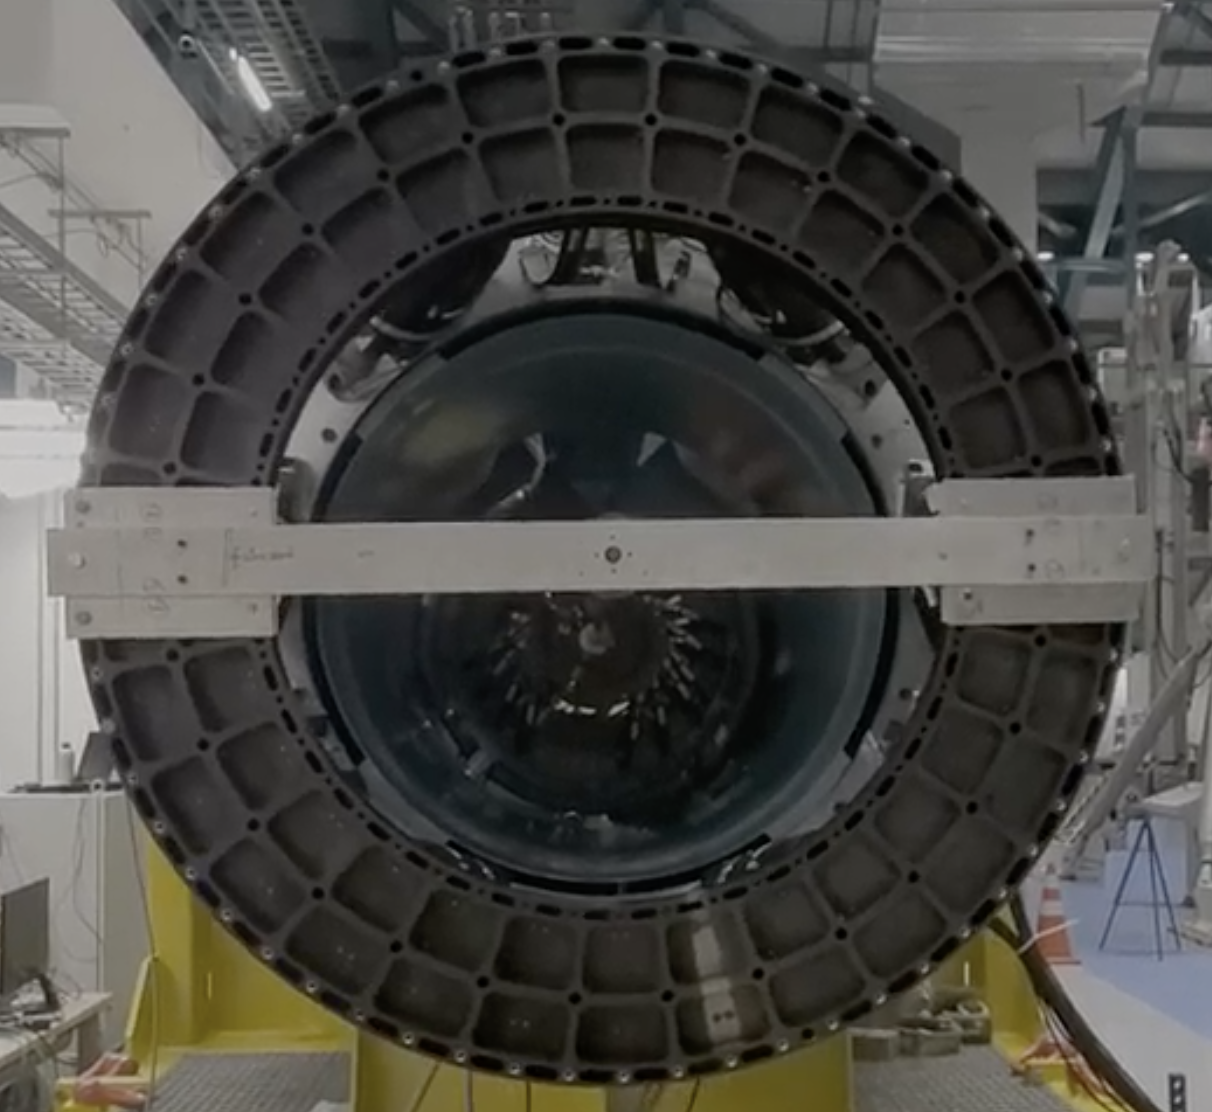
\includegraphics[width=6.5in,height=5.96389in]{media/Figure_2.png}
  \caption{Camera Rotator Temporary Connection Bar}
  \label{fig:Figure_2}
\end{figure}

\subsection{Objective}

The objective of this characterization is to find the allowable position
range of the positive and negative limit switches and provide a
recommendation of where they should be positioned. This requires finding
the exact position that the limit switches are currently activated,
finding the back off distance required to release the limit switches,
and finding the maximum distance for the CCW and Camera Rotator to come
to a complete stop after activating the limit switches.

\subsection{Requirements}

The following are the relevant requirements for the synchronous motion
between the CCW and the Camera Rotator.

\underline{LTS-103}

\begin{itemize}
\item
  3.10.13 MCS Camera Cable Wrap Positioning Command

  \begin{itemize}
  \item
    \textbf{Specification:} The camera cable wrap shall be slaved to the
    camera rotator.
  \end{itemize}
\end{itemize}

\underline{LTS-218}

\begin{itemize}
\item
  3.3.7 Rotation Drive Synchronization with Camera Rotator

  \begin{itemize}
  \item
    \textbf{Specification:} During slewing and tracking, the camera
    cable wrap rotation shall remain synchronized with the camera
    rotator to better than 2.2 degrees. An absolute rotation sensing
    encoder shall be incorporated on the rotation drive unit to provide
    position feedback to the telescope control system (TCS).
  \end{itemize}
\item
  3.3.8.1 Slewing Velocity Range

  \begin{itemize}
  \item
    \textbf{Specification:} The rotation drive unit shall be able to
    reach any velocity between 0 and 3.5deg/sec with a goal of
    5.25deg/sec in both rotation directions.
  \end{itemize}
\item
  3.16 Safety Pull Cord

  \begin{itemize}
  \item
    \textbf{Specification}: The functionality of the safety pull-cord
    has been replaced by limit switches now specified in LTS-156.
  \end{itemize}
\item
  3.3.1 Rotation Range

  \begin{itemize}
  \item
    \textbf{Specification:} The camera cable wrap shall be designed to rotate
    over a 180 degree operational range (+/- 90 degrees either side of
    centered position). This 180 degree range must be achievable without
    exceeding any software limit, limit switch or hard stop,
    consequently, an additional 8 degrees (+/-4) is required to
    accommodate these items. The software limits shall limit the motion
    to the 180 degree range. The limit switches shall stop the motion
    within 2 degrees of meeting this maximum operational range. The hard
    stops shall stop the motion within another 2 degrees of the limit
    switches.
  \end{itemize}
\end{itemize}

\underline{LTS-156}

\begin{itemize}
\item
  The limits shall be adjusted to nominally stop rotation for any twist
  between the bulkhead plate and the wobble plate greater than +/- 3.5
  degrees with adjustment range from 2.5 degrees to 5 degrees.
\item
  The limit switch shall be tested over the range of travel of the
  wobble plate as specified below.

  \begin{itemize}
  \item
    The wobble plate radial motion is +/- 110mm.
  \item
    The wobble plate tilt about its center is +/- 3 degrees.
  \item
    The wobble plate Z motion is +/- 15mm.
  \end{itemize}
\end{itemize}

\underline{LTS-206}

\begin{itemize}
\item
  3.4.5.1 Rotator Slewing Velocity Range

  \begin{itemize}
  \item
    \textbf{Specification:} During a rotator slew, the Camera Rotator
    shall be able to reach any velocity between 0 and 3.5deg/sec with a
    goal of 5.25deg/sec in both rotation directions.
  \end{itemize}
\item
  3.4.4 Rotator Rotation Range

  \begin{itemize}
  \item
    \textbf{Specification:} The Camera Rotator shall be designed to
    rotate over a 180 degree operational range (+/-90 degrees TBR). This
    range must be achievable without reaching any software limit, limit
    switch or hard stop. The limit switches shall stop the motion within
    2 degrees of meeting this maximum operational range. The hard stops
    shall be within another 2 degrees of the limit switches.
  \end{itemize}
\end{itemize}

\underline{LSE-80}

\begin{itemize}
\item
  CA-TS-MEC-ICD-0058 Maximum Allowed Camera Motion at Bulkhead Plate

  \begin{itemize}
  \item
    \textbf{Specification:} The telescope shall ensure that the maximum
    transverse and axial motions of the back end of the camera utility
    trunk are no larger than \textbf{UTradialMotion} transverse,
    \textbf{UTaxialMotion} axial load, and \textbf{UTrotMotion} angular
    rotation around a radial line.
  \item
    UTrotMotion = 5 degrees
  \end{itemize}
\end{itemize}

\section{Characterization Tasks}\label{sec:Characterization Tasks}

The following sections define the tasks that were performed, the details
of how they were performed, and the results of the task.

\subsection{Positive Limit Switch Activation Location}

To determine the exact location that the cam activates the positive
limit switch we moved the CCW slowly and in small increments to find
where the interlock was activated. We moved the CCW at a velocity of 0.1
deg/s and in 0.05 deg increments. This was only performed with the CCW
as it should not matter which system is used to activate the limit
switches at this low velocity and increments.

The positive limit switch was activated at \textbf{+6.16 deg}.

\subsection{Positive Limit Switch Release Location}

To determine where the positive limit switch is released, we first moved
the CCW slowly and in small increments to find where the interlock was
released. We moved the CCW at a velocity of 0.1 deg/s and in 0.05 deg
increments. This was only performed with the CCW because the CCW has the
override for the interlock and is defined to be the system used to
release the limit switch.

The positive limit switch was released at \textbf{+3.11 deg}.

Next, we moved at the design velocity of 3.5 deg/s in a single move in
the releasing direction to find where the limit switch is released which
is a real-world way that we would release the interlock. At these small
distances the velocity never reached the full design velocity. Each time
the limit switch was activated, we did a single move in the releasing
direction increasing by 0.05 deg until we found the location that the
limit switch was released.

The positive limit switch was released at \textbf{+3.06 deg}.

\subsection{Positive Limit Switch CCW Design Velocity Stopping Distance}

To determine the CCW stopping distance for the design velocity after
activating the positive limit switch we moved the CCW in the positive
direction with enough distance to reach a velocity of 3.5 deg/s before
activating the limit switch. This was repeated 10 times. It was
identified after the CCW runs were completed that the Rotator was not
positioned at 0 deg as we thought. We adjusted the stopping distance
values to account for the Rotator being positioned at -1.16 deg instead
of being positioned at 0 deg. We ran an additional 10 runs with the
Rotator positioned at 0 deg and validated that adjusting the values for
the first set 10 runs are in line with the second set of 10 runs. To
calculate the stopping distance after activation we subtracted the
activation location determined in Section 3.1 from the position the CCW
came to a complete stop.

The maximum stopping distance after activating the positive limit switch
was found to be \textbf{0.23 deg}. See Appendix A for the data points
and Appendix B for the EFD data.

\subsection{Positive Limit Switch CCW Goal Velocity Stopping Distance}

To determine the CCW stopping distance for the goal velocity after
activating the positive limit switch we moved the CCW in the positive
direction with enough distance to reach a velocity of 5.0 deg/s before
activating the limit switch. This was repeated 10 times. It was
identified after the CCW runs were completed that the Rotator was not
positioned at 0 deg as we thought. We adjusted the stopping distance
values to account for the Rotator being positioned at -1.16 deg instead
of being positioned at 0 deg. While the goal velocity requirement is
5.25 deg/s the limit was already set to 5.0 deg/s in the CCW so we used
that instead of changing the configuration. We were interested in the
goal velocity of the CCW since the CCW is now following the Rotator and
there is still a possibility that could drive the CCW to require a
higher limit than the design velocity. To calculate the stopping
distance after activation we subtracted the activation location
determined in Section 3.1 from the position the CCW came to a complete
stop.

The maximum stopping distance after activating the positive limit switch
was found to be \textbf{0.35 deg}. See Appendix A for the data points
and Appendix B for the EFD data.

\subsection{Positive Limit Switch Camera Rotator Design Velocity Stopping Distance}

To determine the Rotator stopping distance for the design velocity after
activating the positive limit switch we moved the Rotator in the
negative direction with enough distance to reach a velocity of 3.5 deg/s
before activating the limit switch. Since we defined the positive limit
switch to be the limit switch that is activated by the CCW moving in the
positive direction this correlates to the Rotator moving in the negative
direction. This was repeated 10 times. To calculate the stopping
distance after activation we subtracted the activation location
determined in Section 3.1 from the position the Rotator came to a
complete stop.

The maximum stopping distance after activating the positive limit switch
was found to be \textbf{0.14 deg}. See Appendix A for the data points
and Appendix B for the EFD data.

We did not find the stopping distance with the Rotator at the goal
velocity because the limit was set in the configuration file and there
are no plans to use the Rotator above the design velocity limit.

\subsection{Negative Limit Switch Activation Location}

To determine the exact location that the cam activates the negative
limit switch we moved the CCW slowly and in small increments to find
where the interlock was activated. We moved the CCW at a velocity of 0.1
deg/s and in 0.05 deg increments.

The negative limit switch was activated at \textbf{-2.99 deg}.

\subsection{Negative Limit Switch Release Location}

To determine where the negative limit switch is released, we first moved
the CCW slowly and in small increments to find where the interlock was
released. We moved the CCW at a velocity of 0.1 deg/s and in 0.05 deg
increments. This was only performed with the CCW because the CCW has the
override for the interlock and is defined to be the system used to
release the limit switch.

The negative limit switch was released at \textbf{+0.31 deg}.

Next, we moved at the design velocity of 3.5 deg/s in a single move in
the releasing direction to find where the limit switch is released which
is a real-world way that we would release the interlock. At these small
distances the velocity never reached the full design velocity. Each time
the limit switch was activated, we did a single move in the releasing
direction increasing by 0.05 deg until we found the location that the
limit switch was released. This was repeated several times starting at
various distances from the limit switch when activating the limit switch
to see if the velocity to which the limit switch was activated
influences the distance required to release the limit switch.

The negative limit switch was released at \textbf{+0.30 deg}. We found
that the velocity at which the limit switch was activated did have and
effect on the releasing distance but it was not linear. We found that
there was a distance of approximately 3 deg from the limit switch where
the releasing distance required changed by 0.05 deg. We did not explore
this any further as it is not really relevant for this characterization
as we will take the maximum value.

\subsection{Negative Limit Switch CCW Design Velocity Stopping Distance}

To determine the CCW stopping distance for the design velocity after
activating the negative limit switch we moved the CCW in the negative
direction with enough distance to reach a velocity of 3.5 deg/s before
activating the limit switch. This was repeated 10 times. It was
identified after the CCW runs were completed that the Rotator was not
positioned at 0 deg as we thought. We adjusted the stopping distance
values to account for the Rotator being positioned at -1.16 deg instead
of being positioned at 0 deg. We ran an additional 10 runs with the
Rotator positioned at 0 deg and validated that adjusting the values for
the first set 10 runs are in line with the second set of 10 runs. To
calculate the stopping distance after activation we subtracted the
activation location determined in Section 3.6 from the position the CCW
came to a complete stop.

The maximum stopping distance after activating the negative limit switch
was found to be \textbf{0.23 deg}. See Appendix A for the data points
and Appendix B for the EFD data.

\subsection{Negative Limit Switch CCW Goal Velocity Stopping Distance}

To determine the CCW stopping distance for the goal velocity after
activating the negative limit switch we moved the CCW in the negative
direction with enough distance to reach a velocity of 5.0 deg/s before
activating the limit switch. This was repeated 10 times. It was
identified after the CCW runs were completed that the Rotator was not
positioned at 0 deg as we thought. We adjusted the stopping distance
values to account for the Rotator being positioned at -1.16 deg instead
of being positioned at 0 deg. While the goal velocity requirement is
5.25 deg/s the limit was already set to 5.0 deg/s in the CCW so we used
that instead of changing the configuration. We were interested in the
goal velocity of the CCW since the CCW is now following the Rotator and
there is still a possibility that could drive the CCW to require a
higher limit than the design velocity. To calculate the stopping
distance after activation we subtracted the activation location
determined in Section 3.6 from the position the CCW came to a complete
stop.

The maximum stopping distance after activating the negative limit switch
was found to be \textbf{0.34 deg}. See Appendix A for the data points
and Appendix B for the EFD data.

\subsection{Negative Limit Switch Camera Rotator Design Velocity Stopping Distance}

To determine the Rotator stopping distance for the design velocity after
activating the negative limit switch we moved the Rotator in the
positive direction with enough distance to reach a velocity of 3.5 deg/s
before activating the limit switch. Since we defined the negative limit
switch to be the limit switch that is activated by the CCW moving in the
negative direction this correlates to the Rotator moving in the positive
direction. This was repeated 10 times. To calculate the stopping
distance after activation we subtracted the activation location
determined in Section 3.6 from the position the Rotator came to a
complete stop.

The maximum stopping distance after activating the negative limit switch
was found to be \textbf{0.36 deg}. See Appendix A for the data points
and Appendix B for the EFD data.

We did not find the stopping distance with the Rotator at the goal
velocity because the limit was set in the configuration file and there
are no plans to use the Rotator above the design velocity limit.

\begin{landscape}
\section{Recommendations}

\subsection{Characterization Results}

The tables below provides a summary of the calculations performed on the
data captured to determine the result of the tasks define in Section \ref{sec:Characterization Tasks}.

\begin{table}[h!]
  \begin{center}
    \caption{CCW Positive Limit Switch Characterization Calculation Results}
    \label{tab:table1}
    \begin{tabular}{r|c|r|c|r|c|c|c}
    \multicolumn{5}{l|}{\textbf{CCW Positive Limit Switch}} & Avg & Max & Std Dev\\
    \midrule
    Activation location: & 6.16 & & & & & & \\
    Release location: & 3.11 & Single motion release location: & 3.06 & 3.5
    deg/s stopping location: & 6.366 & 6.39 & 0.01284 \\
    Incremental delta: & 3.05 & Single motion delta: & 3.10 & 5.0 deg/s
    stopping location: & 6.478 & 6.51 & 0.01778 \\
    & & & & 3.5 deg/s stopping distance: & 0.206 & \textbf{0.23} & \\
    & & & & 5.0 deg/s stopping distance: & 0.318 & \textbf{0.35} & \\
    \end{tabular}
  \end{center}
\end{table}

\begin{table}[h!]
  \begin{center}
    \caption{CCW Negative Limit Switch Characterization Calculation Results}
    \label{tab:table2}
    \begin{tabular}{r|c|r|c|r|c|c|c}
    \multicolumn{5}{l|}{\textbf{CCW Negative Limit Switch}} & Avg & Max & Std Dev\\
    \midrule
    Activation location: & -2.99 & & & & & & \\
    Release location: & 0.31 & Single motion release location: & 0.30 & 3.5
    deg/s stopping location: & -3.190 & -3.22 & 0.01396 \\
    Incremental delta: & 3.30 & Single motion delta: & 3.29 & 5.0 deg/s
    stopping location: & -3.307 & -3.33 & 0.01676 \\
    & & & & 3.5 deg/s stopping distance: & -0.200 & \textbf{ 0.23} & \\
    & & & & 5.0 deg/s stopping distance: & -0.317 & \textbf{ 0.34} & \\
    \end{tabular}
  \end{center}
\end{table}

\begin{table}[h!]
  \begin{center}
    \caption{Rotator Positive Limit Switch Characterization Calculation Results}
    \label{tab:table3}
    \begin{tabular}{r|c|r|c|c|c}
    \multicolumn{3}{l|}{\textbf{Rotator Positive Limit Switch}} & Avg & Max & Std Dev\\
    \midrule
    Activation location: & -6.16 & & & & \\
    & & 3.5 deg/s stopping location: & -6.28 & -6.30 & 0.01549 \\
    & & 5.0 deg/s stopping location: & N/A & N/A & N/A \\
    & & 3.5 deg/s stopping distance: &  0.12 & \textbf{ 0.14} & \\
    & & 5.0 deg/s stopping distance: & N/A & \textbf{N/A} & \\
    \end{tabular}
  \end{center}
\end{table}

\begin{table}[h!]
  \begin{center}
    \caption{Rotator Negative Limit Switch Characterization Calculation Results}
    \label{tab:table4}
    \begin{tabular}{r|c|r|c|c|c}
    \multicolumn{3}{l|}{\textbf{Rotator Negative Limit Switch}} & Avg & Max & Std Dev\\
    \midrule
    Activation location: & 2.99 & & & & \\
    & & 3.5 deg/s stopping location: & 3.283 & 3.35 & 0.03035 \\
    & & 5.0 deg/s stopping location: & N/A & N/A & N/A \\
    & & 3.5 deg/s stopping distance: & 0.293 & \textbf{0.36} & \\
    & & 5.0 deg/s stopping distance: & N/A & \textbf{N/A} & \\
    \end{tabular}
  \end{center}
\end{table}

\end{landscape}

\subsection{Limit Switch Activation Location Recommendation}

Based on the maximum distance required to release the limit switch the
closest activation location, with no margin, would be +/- 3.3 deg
without activating the opposite limit switch. The LSE-80 requirement for
the angular rotation between the bulkhead plate and the wobble plate is
5 degrees so that should be the minimum slack in the utility lines and
the maximum angular rotation between the CCW and the Rotator after
activating the limit switch and coming to a complete stop.

Based on the requirements and characterization of the limit switches we
recommend that the limit switch activation location should be
\textbf{+/- 3.5 deg}.

\subsection{Remaining Work}

Shortly before completing the limit switch characterization it was
identified that the camera team at SLAC had redesigned the bulkhead
plate and how the limit switches and activation cams are connected to
the bulkhead plate. The limit switches have been confirmed to be the
same model as the Tekniker design. See Figure \ref{fig:Figure_3} below for a comparison
of the designs with the Tekniker design on the left and the SLAC design
on the right.

\begin{figure}[h!]
  \centering
  \begin{subfigure}{0.45\linewidth}
    \centering
    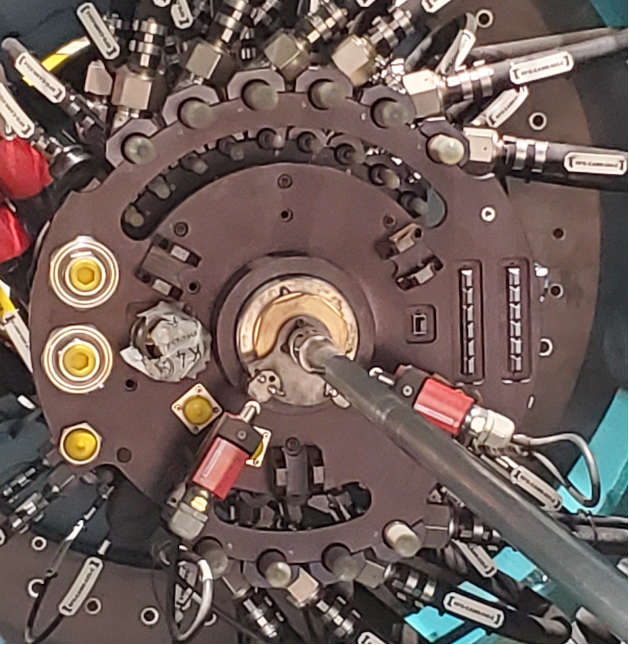
\includegraphics[width=\linewidth]{media/teknikerDesign.png}
    \caption{Tekniker Design}
  \end{subfigure}
  \begin{subfigure}{0.45\linewidth}
    \centering
    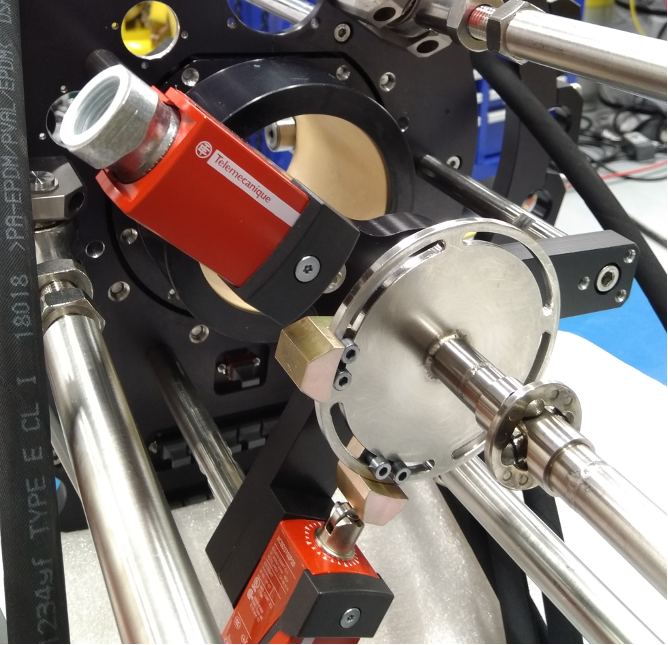
\includegraphics[width=\linewidth]{media/slacDesign.png}
    \caption{SLAC Design}
  \end{subfigure}
  \caption{CCW Bulkhead Deisgn Comparison}
  \label{fig:Figure_3}
\end{figure}

The limit switches have been confirmed to be the same model. The angle
between the limit switches in the Tekniker design and the angle between
the limit switches in the SLAC design have been confirmed to both be 100
deg.

The profile of the detection cams are similar with the same chamfer
angle however the overall width of the cam and the width of the chamfer
is slightly smaller on the SLAC detection cams. See Figure \ref{fig:Figure_4} below for a
comparison of the designs with the Tekniker design (0000053538) on the
left and the SLAC design (LCA-17138) on the right. The impact on the
stopping distance and release location these differences have will need
to be determined.

\begin{figure}[h!]
  \centering
  \begin{subfigure}{0.45\linewidth}
    \centering
    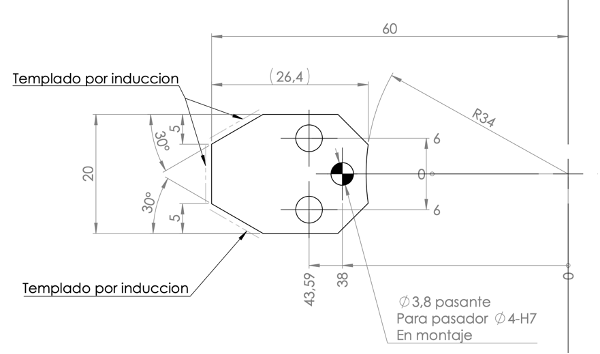
\includegraphics[width=\linewidth]{media/teknikerDrawing.png}
    \caption{Tekniker Design}
  \end{subfigure}
  \begin{subfigure}{0.45\linewidth}
    \centering
    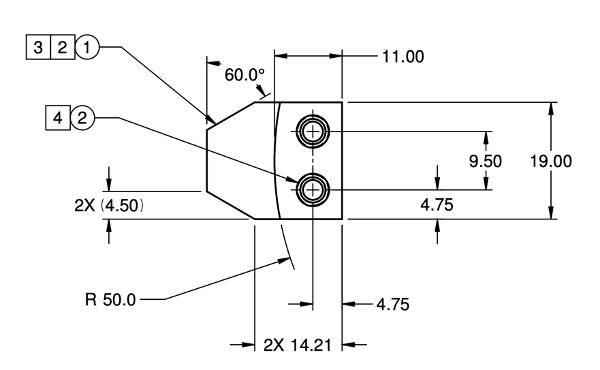
\includegraphics[width=\linewidth]{media/slacDrawing.png}
    \caption{SLAC Design}
  \end{subfigure}
  \caption{Detection Cam Deisgn Comparison}
  \label{fig:Figure_4}
\end{figure}

Due to the differences in the designs of the Tekniker and SLAC bulkhead
plates this characterization will need to be performed again on the SLAC
designed bulkhead plate after being installed with ComCam and before the
utility lines are connected.

Looking at the worst case scenario that could create the maximum angular
difference with the limit switches activated at +/- 3.5 deg would result
in a maximum angular difference of \textbf{5.86 deg}. This scenario
would occur when the CCW activates the end of travel limit switch which
will stop the system within +/- 92 deg and the Rotator activates the
synchronous motion limit switch in the opposite direction which has a
maximum stopping distance of 0.36 deg at approximately the same time.
This compounds to 2 deg + 3.5 deg + 0.36 deg which is the 5.86 deg. This
will need to be recalculated after the characterization of the SLAC
bulkhead plate with ComCam installed so that the Rotator is loaded with
the design mass and CG.

\appendix
\section{Data Points}
\subsection{CCW Positive Limit Switch Data Points}
\subsection{CCW Negative Limit Switch Data Points}
\subsection{Rotator Positive Limit Switch Data Points}
\subsection{Rotator Negative Limit Switch Data Points}

\section{EFD Plots}
% Include all the relevant bib files.
% https://lsst-texmf.lsst.io/lsstdoc.html#bibliographies
\section{References} \label{sec:bib}
\renewcommand{\refname}{} % Suppress default Bibliography section
\bibliography{local,lsst,refs_ads,refs,books}

% Make sure lsst-texmf/bin/generateAcronyms.py is in your path
\section{Acronyms} \label{sec:acronyms}
\input{acronyms.tex}
% If you want glossary uncomment below -- comment out the two lines above
%\printglossaries





\end{document}
